\documentclass[]{article}

\usepackage[UKenglish]{babel}
\usepackage{fullpage}
\usepackage[a4paper, margin=1.2in]{geometry}
\usepackage{amsfonts}
\usepackage{amsmath}
\usepackage{amssymb}
\usepackage{xcolor}
\usepackage{enumitem}
\usepackage{graphicx}
\usepackage{gensymb}
\usepackage{fancyhdr}
\usepackage{times}
%\usepackage{widetext}
\usepackage{ulem}
\usepackage{caption}
%\usepackage{subfigure}
%\usepackage{subcaption}  
\usepackage[caption = false]{subfig}
%\usepackage[draft]{hyperref}
%\usepackage[debug]{hyperref}
%\usepackage{hyperref}
\usepackage{natbib}
%\bibliographystyle{../papers/BibTex/mnras}
\bibliographystyle{apalike}
\usepackage{url}


\title{{\Huge Coffee \& Code:} \\
a guide into the rubbery world of \Huge\LaTeX \ for dummies}
\author{Mr. \& Mrs. Smith}

\begin{document}
\maketitle

\begin{figure}[h!]
\centering
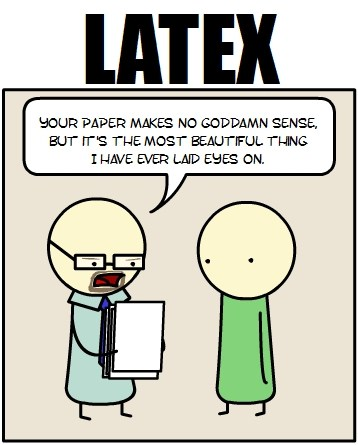
\includegraphics[scale=0.5]{./latex_comic.jpg}
\caption{Warning: This may be may happen to you too if you start using latex...}
\end{figure}


\section*{A few potentially useful links and tips}

A few tips and links.

\begin{itemize}
\item You can use \LaTeX for any sort of document, from papers, to books, to presentations, resumé's, you name it. 
\item \LaTeX is highly flexible, if something is not defined yet (which is possible, although it's also likely that someone already has found a solution to your potential problem), you can program it yourself\footnote{I have never done this yet, but I hear it's possible.. ;-)}! :)
\item Just like with programming, duckduckgo\footnote{In case of no result you may want to resort to the tool from a company that already know way too much about you any way.} and stackoverflow are your friend!
\item to get started, find yourself a good cheat sheet! ({\it hint:} you may have found one already in a convenient location)
\item For collaborative research Overleaf is a great tool to write your paper. But you may find it also useful for yourself. It even has a lot of templates for different journal and direct submit options. See \url{www.overleaf.com}.
\item \LaTeX is open source, so there are many applications or editors to make your documents. I use {\large\bf\TeX Maker} but there's plenty of other options too for various platforms. See \url{https://beebom.com/best-latex-editors/} for a few ideas.
\item citations are hassle free using {\LARGE Bib\TeX}. You can use your favourite paper archive tool such as Mendeley or Citavi to export all your references to a Bib\TeX\ (.bib) file. '
\item Formulas were never as easy to insert and reference!
\item Don't be fooled, there's no such thing as free lunch, \LaTeX can be a pain in the behind at times... :(  But usually the result is great! 
\end{itemize}

Now let's get started! Go to \url{www.overleaf.com} sign in, click \emph{new project}\ :\ \emph{exmaple project} to get started and let's write some document together. You may find a few useful files  in this github folder. 

Oh and one more very useful link:
\begin{center}
{\Large \url{https://en.wikibooks.org/wiki/LaTeX}}
\end{center}

\end{document}